\documentclass{scrartcl}
\usepackage[utf8]{inputenc}
\usepackage[T1]{fontenc}

% Standard ams packages
\usepackage{amsmath}
\usepackage{amssymb}
\usepackage{amstext}

% Für Seitenränder
\usepackage{geometry}
\geometry{
	top=2.5cm,
	left=2.5cm,
	right=2.5cm,
	bottom=2cm,
	includefoot,
	footskip=13.6pt
}

% Für schöneren Blocksatz
\usepackage{microtype}

% Für deutsche Sprache
\usepackage[ngerman]{babel}

% Für deutsche Zitate / Anführungszeichen
\usepackage{csquotes}

% Für Quellenangaben
\usepackage[sorting=none, defernumbers=true]{biblatex}
\addbibresource{sources.bib}

% Für klickbare links (Kasten werden nicht mitgedruckt)
\usepackage[bookmarks=true]{hyperref}
\hypersetup{
	pdftitle={Erkennung ereigniskorrelierte Potenziale eines Elektroenzephalogramms durch eine KI},
	pdfauthor={Matteo Friedrich \& Alexander Reimer},
	pdfsubject={Die Erkennung von Blinzeln in Elektroenzephalogrammen mithilfe von neuronalen Netzwerken},
	pdfkeywords={KI, AI, neuronale Netzwerke, EEG, Elektroenzephalographie, Jugend Forscht, EKP}
}

% Für Zusammenfassung
\usepackage{abstract}

% Für das Einfügen von Bildern
\usepackage{graphicx}

% Für wrapfigure (Text um Bilder herum)
\usepackage{wrapfig}

% Für Einheiten
\usepackage{siunitx}

% Für custom captions
\usepackage{caption}
\captionsetup{textfont={footnotesize}, labelfont={footnotesize, bf}, position=below, format=plain}

% Für \affil
\usepackage{authblk}

\usepackage{float}
% Für Kopf-/Fußzeilen
%\usepackage{scrlayer-scrpage}
% \renewcommand*{\headfont}{\normalfont}
%\setkomafont{pagehead}
%\rehead[]{JUGEND FORSCHT -- PROJEKTBERICHT}
%\rohead[]{JUGEND FORSCHT - PROJEKTBERICHT}


\usepackage{fancyhdr}
\pagestyle{fancy}

\fancyhf{}
\fancyhead[R]{JUGEND FORSCHT -- PROJEKTBERICHT}
\fancyfoot[C]{\thepage}

% Für Seitenränder
% \usepackage{geometry}
% \geometry{left=2.5cm, right=2.5cm, top=2.5cm, bottom=2cm}

\title{\textbf{\Huge 
\texttt{
	Erkennung ereigniskorrelierte Potenziale eines Elektroenzephalogramms durch eine KI
}
} \\ \vspace{15mm}}

\date{}
\author[]{\textbf{\huge Alexander Reimer und Matteo Friedrich}}
\affil[]{\textbf{\LARGE Gymnasium Eversten Oldenburg} \\ \vspace{10mm} \textbf{\Large Betreuer: Herr Dr. Glade \& Herr Husemeyer}}

\begin{document}

	%\setlength{\footskip}{100pt}

	%\renewcommand{\footruleskip}{3cm}

	\newcommand{\sig}{\textrm{sig}}
	\newcommand{\netin}{\textrm{netzinput}}

	\newcommand{\threesub}[1]{
	\vspace{1.5ex}
	\noindent {\textbf{#1}}
	\vspace{0.5ex}
	}

	{\centering

	\vspace*{15mm}
	\textbf{\Huge 
	Erkennung ereigniskorrelierter Potenziale eines Elektroenzephalogramms durch eine KI
	}

	\vspace{15mm}

	\textbf{\huge Alexander Reimer und Matteo Friedrich}

	\vspace{1em}

	\textbf{\LARGE Gymnasium Eversten Oldenburg}

	\vspace{10mm}

	\textbf{\Large Betreuer: Herr Dr. Glade \& Herr Husemeyer}

	\vspace{20mm}

	
\includegraphics[width=0.8\textwidth]{pictures/logo.png}

	}

	\newpage
	
	\tableofcontents
	
	\newpage

	\section{Kurzfassung}


	In diesem Projekt wollen wir einen Roboter mithilfe bloßer Gedankenkraft steuern.

	Um Daten über das Gehirn zu bekommen, nutzen wir einen Elektroenzephalographen, kurz EEG, welches durch Elektroden an der Kopfhaut die Spannungsdifferenzen innerhalb des Gehirns misst. Diese werten wir mithilfe eines neuronalen Netzes aus, welches wir vorher darauf trainiert haben, Muster in diesen Daten zu erkennen. So können wir bestimmte Ereignisse anhand der EEG-Daten ableiten, z.B. ob jemand geblinzelt hat oder sich gerade konzentriert.
	
	Das Ziel ist es dann, einen Roboter nur mit Gedanken steuern zu können.
	
	Wir haben bereits ein geeignetes neuronales Netz trainiert, welches Blinzeln sicher erkennen kann. Die Steuerung eines Roboters funktioniert ebenfalls.
	
	Wir hoffen, in Zukunft den Roboter auch durch Gedanken an bestimmte Richtungen und nicht nur Blinzeln steuern zu können.

	\section{Einleitung}

	Ziel des Projektes ist es, zuerst ein BCI -- Brain-Computer-Interface -- zu entwickeln, welches verschiedene EKPs erkennen kann. Dieses wollen wir dann testen, indem wir es zur Steuerung eines Roboters nutzen.

	Die Idee eines BCI ist nicht neu, sondern wird intensiv erforscht. Aufgrund bereits durchgeführter Experimente ist bekannt, dass BCIs umsetzbar sind \cite{BCIChaudhary}.
	
	Wir hoffen, neben dem Erlangen von Erfahrung in diesem interessanten Bereich auch selbst dazu beizutragen. Dies wollen wir erreichen durch das Entwickeln einer allgemeinen Anwendung, bei der kein vorheriges Trainieren für eine fremde Person benötigt wird, das Umsetzen mit günstiger, für viele bezahlbare Hardware, sowie ein performantes Programm, welches leicht für die eigenen Zwecke anpassbar ist.

	\section{Methode und Vorgehensweise}

	\subsection{Materialien} \label{Materialien}

	\begin{itemize}
		\item EEG
		\begin{itemize}
			\item 4 Channel Ganglion Board von OpenBCI $\star$
			\item 2x Spike und 2x Flat Electrodes  $\star$
			\item Klettband für die Elektroden $\star$
			\item 2x Earclips $\star$
			\item Lithium-Polymer-Akku und Ladegerät $\star$
			\item Plastik-Hülle für das Ganglion Board
		\end{itemize}
		\item Roboter
		\begin{itemize}
			\item Lego Mindstorms EV3 Brick
			\item Raspberry Pi 3B 8\,GB
			\item 2x EV3 großer Motor
			\item SD-Karte (8\,GB)
			\item diverse LEGO Teile
		\end{itemize}

		\item Computer: Aorus 15P
		\begin{itemize}
			\item CPU: i7-11800H
			\item GPU: RTX 3060
			\item RAM: 16\,GB
		\end{itemize}

		\item Software
		\begin{itemize}
			\item Flux.jl für das neuronale Netz
				\footnote{\href{https://github.com/FluxML/Flux.jl}{https://github.com/FluxML/Flux.jl}}
				\cite{Flux.jl-2018}
				\cite{innes:2018}
			
			\item BrainFlow.jl als Schnittstelle zum EEG
				\footnote{\href{https://github.com/brainflow-dev/brainflow}{https://github.com/brainflow-dev/brainflow}}
				\cite{brainflow}
			
			\item FFTW.jl für die Fast Fourier Transformation
				\footnote{\href{https://github.com/JuliaMath/FFTW.jl}{https://github.com/JuliaMath/FFTW.jl}}
				\cite{FFTW.jl-2005}
			
			\item CUDA.jl zum effektiven Nutzen einer NVIDIA GPU
				\footnote{\href{https://github.com/JuliaGPU/CUDA.jl}{https://github.com/JuliaGPU/CUDA.jl}}
				\cite{CUDA}
			
			\item PyPlot.jl zum Plotten
				\footnote{\href{https://github.com/JuliaPy/PyPlot.jl}{https://github.com/JuliaPy/PyPlot.jl}}
				\cite{pyplot}
			
			\item BSON.jl zum Speichern und Laden von Netzwerken
				\footnote{\href{https://github.com/JuliaIO/BSON.jl}{https://github.com/JuliaIO/BSON.jl}}
			
			\item ev3dev.jl zum Steuern eines EV3-Roboters durch einen Raspberry Pi
				\footnote{\href{https://github.com/AR102/ev3dev.jl}{https://github.com/AR102/ev3dev.jl}}
				\cite{ev3dev}
			
		\end{itemize}

	\end{itemize}

	\begin{figure}[h!]
		\includegraphics[width=0.5\textwidth]{pictures/EEG-Alex-annotated.png}
		\includegraphics[width=0.35\textwidth]{pictures/Ganglion-Board-annotated.png}
		\caption{Das EEG und Zubehör}
		\label{EEG-Zubehor}
	\end{figure}

	Unser EEG-Gerät besteht aus einem Klettband mit Löchern für die Elektroden, einer Platine (Ganglion Board), in welche die Elektroden eingesteckt werden, einer Kunststoff-Hülle zum Schutz des Ganglion Boards, und einem USB-Dongle, mit welchem die Signale der Platine kabellos empfangen werden können (s. Abbildung \ref{EEG-Zubehor}).

	\subsection{Vorgehensweise}

	Unser Projekt lässt sich grob in 3 Teile unterscheiden.

	Zum einen gibt es den neurobiologischen Teil. Dieser besteht aus der Messung von Gehirnaktivität und der Umwandlung dieser Aktivität in für uns nutzbare Daten.
	
	Der zweite Teil besteht aus der Verarbeitung dieser Signale. Hierfür nutzen wir ein neuronales Netz, welches Muster in den Gehirnaktivitäten erkennen kann.
	
	Der letzte Teil von unserem Projekt beinhaltet die Konstruktion und Steuerung eines EV3 Roboters. Je nachdem, was das neuronale Netz ausgibt, soll sich dieser Roboter anders verhalten und so über Gedanken steuerbar sein.	

	\subsubsection{Elektroenzephalographie}

	Bei der Elektroenzephalographie (EEG) werden Elektroden an der Kopfoberfläche platziert. Diese können sehr kleine Spannungsdifferenzen messen, die durch Reize im Gehirn entstehen und durch den Schädel dringen. Diese Spannungen werden nicht von einzelnen Nervenzellen erzeugt, sondern geben die Summe aller lokalen Spannungen wieder. Man kann also auch nur ungefähr sagen, wo genau im Gehirn ein bestimmter Reiz ausgelöst wurde, je mehr Elektroden, desto höher die Genauigkeit. \cite{wiki:EEG}

	Wir untersuchen dabei ereigniskorrelierte Potentiale (EKPs). Dies sind bestimmte Spannungsschwankungen (\enquote{Potentiale}), welche in Zusammenhang mit einem beobachtbaren Ereignis stehen, wie z.B. Blinzeln oder Armbewegungen. \cite{Birbaumer2010} \cite{Praktikum}

	Dabei haben wir uns für das Blinzeln entschieden, da wir es im Graphen zumindest mit bloßen Augen sehr gut erkennen konnten (s. Abbildung \ref{EEG-Blinzeln}).

	\begin{figure}[h]
		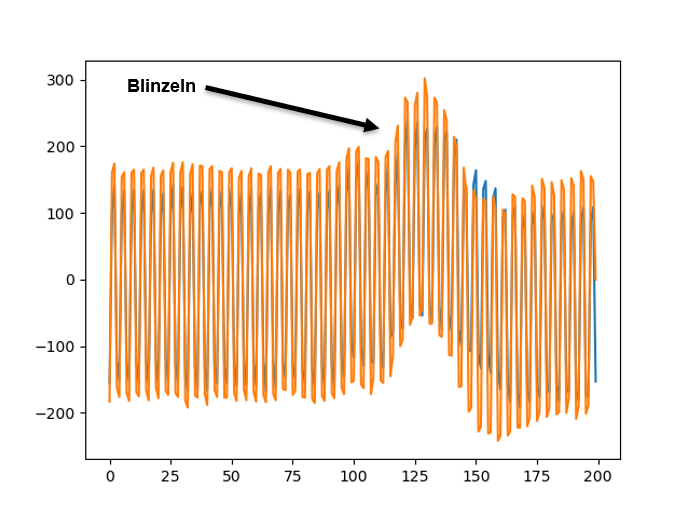
\includegraphics{pictures/blinzeln_ekp_beispiel_pyplot_annotated.png}
		\caption{Ausschnitt eines EEG mit Blinzeln}
		\label{EEG-Blinzeln}
	\end{figure}

	Für unser Projekt nutzen wir zwar die Ausrüstung für EEG, aber genau genommen wird das Blinzeln mithilfe von Elektromyographie (EMG) erkannt, denn aufgrund der Platzierung der zwei verwendeten Elektroden direkt über den Augen werden nicht die Spannungsdifferenzen des Gehirns gemessen, sondern die für das Blinzeln verantwortlichen Augenmuskeln \cite{wiki:EMG}.

	Wir haben uns für diesen Anfang entschieden, da im EMG ein Blinzeln sehr sicher erkennbar ist und wir so eine mangelnde Genauigkeit des Messgerätes als Fehlerquelle ausschließen konnten, solange wir noch an dem neuronalen Netz und der Datenverarbeitung arbeiten.

	%Da wir nun wissen, dass diese Komponenten im Kern funktionieren, wollen wir die Elektroden am Hinterkopf, genauer dem Okzipitale Kortex, platzieren, sodass wir tatsächlich die Potentiale des Gehirns messen und somit unser Ziel der Deutung eines Elektroenzephalogramms erreichen können.

	Weiter ist es möglich, nur durch Gedanken eine Steuerung auszuführen. Dies funktioniert jedoch meist durch instrumentelle oder klassische Konditionierung, also durch das Bestrafen und Belohnen auf Basis der Messungen des EEG. So kann das Gehirn darauf trainiert werden, auf Verlangen eine bestimmte, vorher festgelegte Aktivität auszulösen, die dann gemessen und ausgewertet werden kann. \cite{BCIChaudhary}

	Darauf wollen wir erstmal verzichten, da die Konditionierung Zeit benötigen und nicht unser Ziel einer allgemeinen Anwendbarkeit erfüllen würde.

	Insgesamt haben wir zwei Earclips, die an den Ohren befestigt werden und zum Filtern von Störungen dienen, und vier Messelektroden, mit einer zeitlichen Auflösung von jeweils 200 Hertz (200 Messungen pro Sekunde).

	Zwei dieser Elektroden haben wir auf der Stirn platziert (links: Elektrode 1, rechts: Elektrode 2), zwei jeweils links (Elektrode 3) und rechts (Elektrode 4) auf dem Schädel, etwas über und vor dem Ohr (s. Abbildung \ref{10-20-System}). Wir haben uns für diese Platzierung entschieden, da die Elektroden so direkt über Muskeln sitzen, die beim Blinzeln bewegt werden. %!!!

	\begin{figure}[h!]
		\centering
		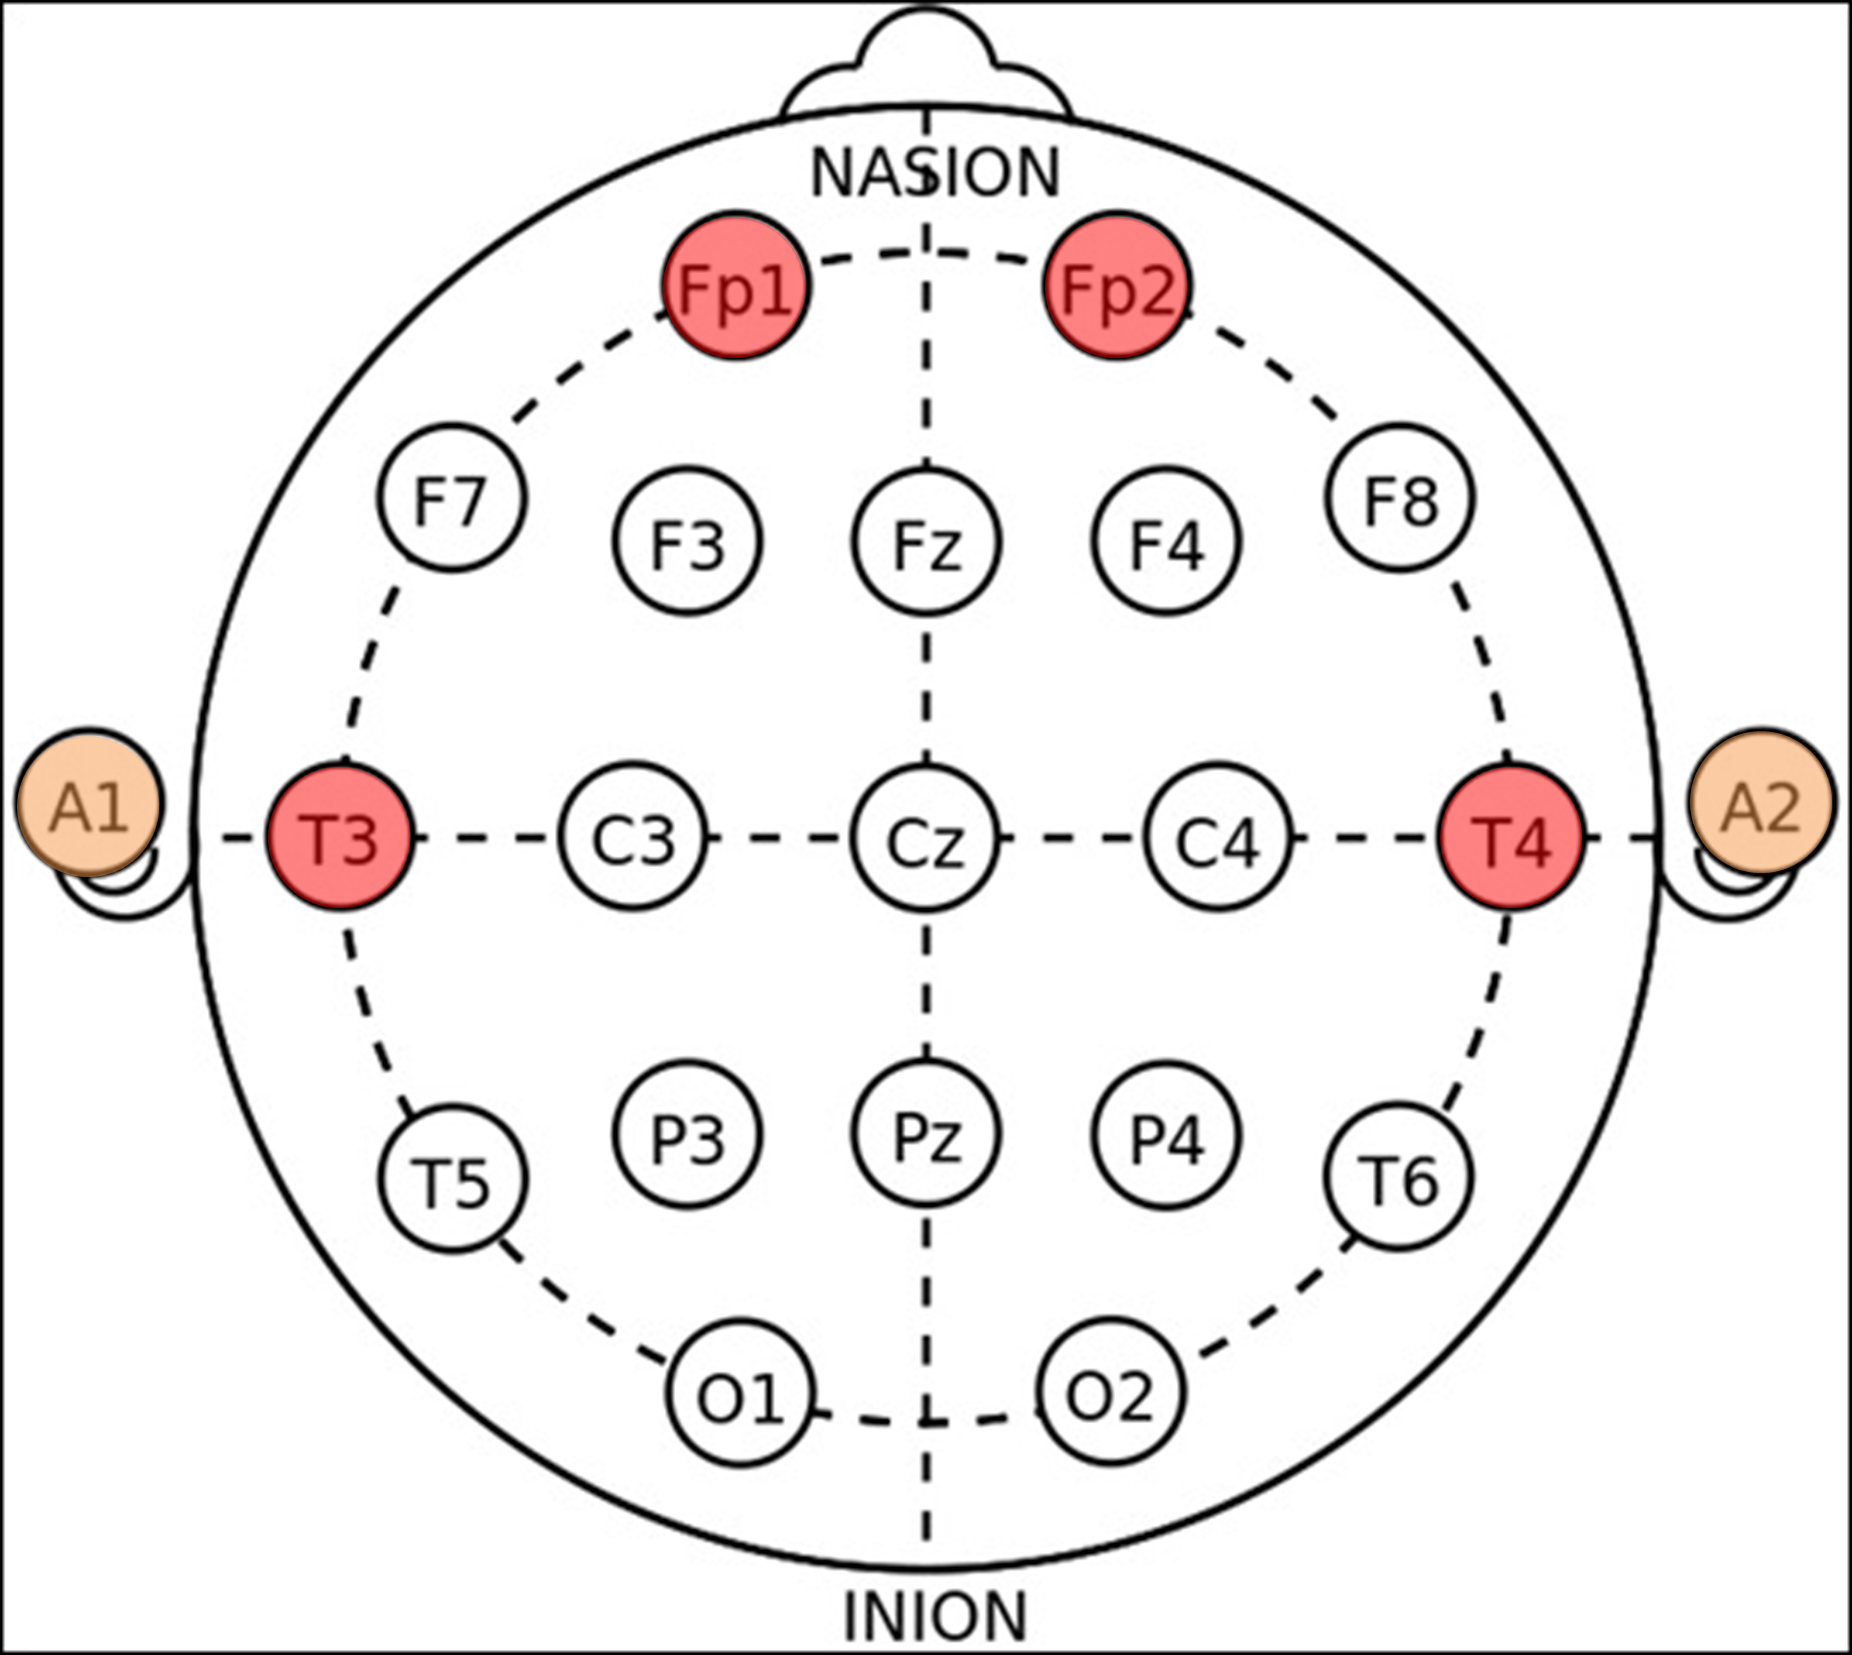
\includegraphics[width=0.5\textwidth]{pictures/elektroden-platzierungen.png}
		\caption{10-20 System mit den von uns genutzten Elektroden rot und Earclips orange gefärbt}
		\label{10-20-System}
	\end{figure}

	Uns ist nach der Aufnahme der Trainingsdaten aufgefallen, dass die Elektroden 3 und 4 deutlich schlechtere Signalqualität hatten als Elektroden 1 und 2, vermutlich weil die Elektroden 3 und 4 auf Haaren auflagen und weiter von den Augen entfernt waren.

	Deswegen haben wir uns entschieden, nur die Elektroden 1 und 2 zu verwenden.

	Also kriegen wir $2 * 200 = 400$ Signale pro Sekunde.

	\subsubsection{Fourier-Analyse}
	
	Uns wurde von Professor Everling (s. Danksagung) empfohlen, die Anwendung der Fourier-Analyse zur Vorbereitung der Daten für das neuronale Netz zu bedenken.
	
	Die Fourier-Analyse kann die verschiedenen zugrundeliegenden Frequenzen von Datenfolgen, Funktionen, und mehr bestimmen, indem diese in Sinus-Kurven zerlegt werden, sie dient also zur Spektralanalyse \cite{3b1b:fft}.

	Wir nutzen dafür die Fast Fourier Transformation (FFT), welche lediglich eine komplexere aber effizientere Form der Diskreten Fourier Transformation (DFT) ist \cite{FFT-DFT}.

	%Grund für die Verwendung einer DFT ist, dass wir ein zeitdiskretes endliches Signal haben, also eine endliche Anzahl (200 pro Elektrode) an Datenpunkten, die auf konkrete Zeitpunkte bezogen sind, und keine unendlichen (iterativen) Funktionen.

	Aus der FFT folgt ein Array (eine Liste) an Werten. Der Index dieser Liste bestimmt, für welche Frequenz der Wert gilt (erster Wert: 1 Hertz, zweiter Wert: 2 Hertz, etc.) und der Wert gibt die Amplitude der entsprechenden Sinus-Kurve an \cite{3b1b:fft}.

	So lässt sich bestimmen, welche Frequenzen am stärksten vorkommen. Außerdem können dann Frequenzen herausgefiltert werden, indem die entsprechenden Indices ignoriert werden.

	Eine FFT kann Elektroenzephalogramme fast verlustfrei repräsentieren. Dies lässt sich erkennen, wenn man mithilfe der durch die FFT entstandenen Spektralanalyse die Daten rekonstruiert (Inverse Fast Fourier Transformation, IFFT) (s. Abbildung \ref{EEG-IFFT}). Dazu werden die Sinus-Kurven der Frequenzen mit den entsprechenden Amplituden multipliziert und dann addiert.

	\begin{figure}[h!]
		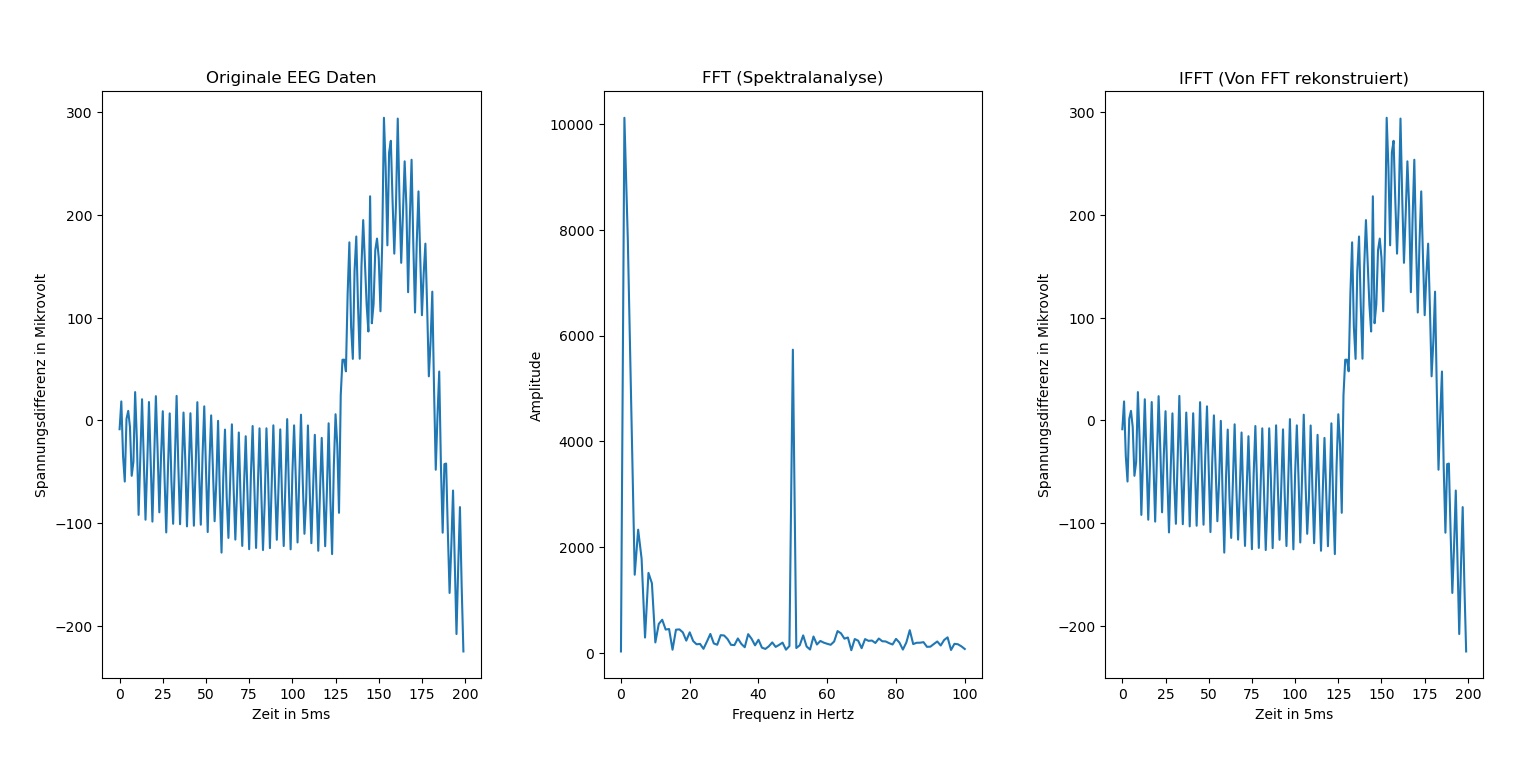
\includegraphics[width=\textwidth]{pictures/blink_fft_ifft.png}
		\caption{Das EEG eines Blinzelns, eine FFT dessen, und eine IFFT}
		\label{EEG-IFFT}
	\end{figure}

	Aber vor der Implementation haben wir getestet, ob eine Spektralanalyse für unseren Zweck überhaupt sinnvoll ist. Dazu haben wir die Ergebnisse der FFT von Elektroenzephalogrammen mit Blinzeln und ohne Blinzeln verglichen. Wie man in Abbildung \ref{EEG-FFT} sehen kann, gibt es vor allem im niedrigeren Frequenzbereich einen klaren Unterschied. % Grund dafür ist wahrscheinlich, dass die Qualität unseres EEG beschränkt ist und es höhere Frequenzbereiche deswegen nicht so gut aufzeichnen kann, da diese nicht so leicht durch den Schädel dringen können.
	Somit ist es geeignet, da die KI in der Lage sein sollte, diesen Unterschied zu erkennen.

	\begin{figure}[H]
		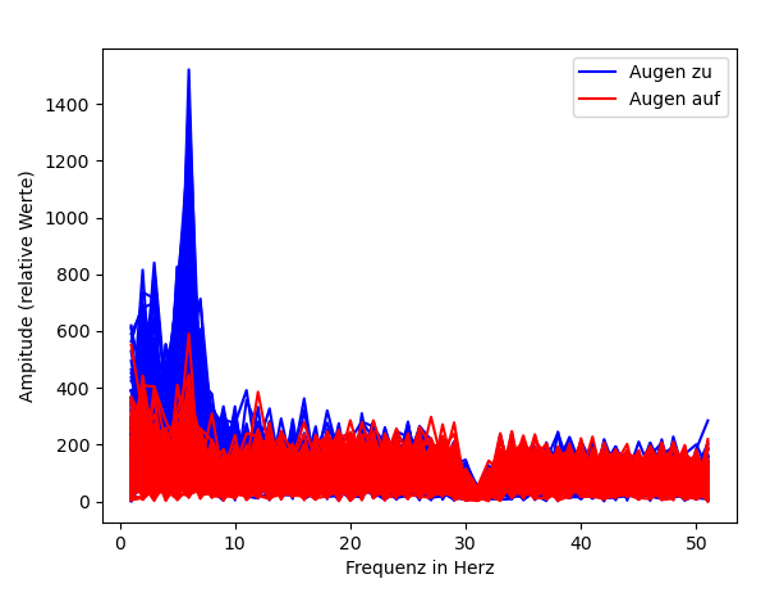
\includegraphics[width=0.9\textwidth]{pictures/Die_FFTs_der_EEG-Daten.png}
		\caption{Die FFT unserer EEG-Daten}
		\label{EEG-FFT}
	\end{figure}
	
	Ob FFT einen Vorteil zu den rohen Daten darstellen wird, werden wir in den Ergebnissen sehen müssen, jedoch liegt es nahe, da die KI sich auf einige wenige, wichtige Inputs konzentrieren kann. Denn wie man sehen kann, ist der Unterschied in den höheren Frequenzen nicht so groß und vermutlich für eine sichere Erkennung nicht unbedingt notwendig.

	Die große Amplitude bei 50 Hertz ist aufgrund der Verstrahlung der Umgebung, die meist besonders die Frequenz von 50 Hertz betrifft \cite{Praktikum}. % Quelle überprüfen!

	Um eine Verwirrung der KI zu verhindern, können wir bei Verwendung von FFT also auch einfach die Amplitude für 50 Hertz auf 0 setzen.

	Die FFT ist außerdem sehr schnell, auf unserem Test-System braucht sie für die Verarbeitung von einer Sekunde Messdaten von zwei Elektroden im Schnitt \qty{22}{\micro\second}.

	Ein weiterer Vorteil der FFT ist, dass wir weniger Inputs haben. Denn wir brauchen aller höchstens die Amplituden für 1-100 Hertz, alles darüber kann unser EEG sowieso nicht akkurat wahrnehmen. Mit 100 Inputs (die Frequenzen) statt 200 Inputs (jede einzelne Spannungsdifferenz) kann unsere KI schneller lernen und schneller eine Erkennung durchführen.

	Dennoch wollen wir das Programm auch ohne FFT ausprobieren -- wenn die Ergebnisse gleich gut sind, würde es sich trotzdem lohnen, auf FFT zu verzichten, da für FFT auch die Installation eines weiteren Packages (FFTW) notwendig ist. 

	\subsubsection{Neuronales Netz}

	Ein neuronales Netzwerk besteht aus drei Teilen: dem Input Layer, den Hidden Layers und dem Output Layer.

	Der Input Layer ist eine Liste aus Zahlen zwischen 0 und 1. Er gibt an, welche Eingaben (Inputs) das Netzwerk bekommen soll, z. B. die Grauwerte der Pixel eines Bildes.
	
	Die Hidden Layers sind eine Ansammlung von in mehrere Layer (Schichten) unterteilten Neuronen.
	
	Jedes Neuron besitzt eine Aktivierung (Activation), die als Zahl zwischen 0 und 1 angegeben werden kann, und einen Bias (Verzerrung), der eine beliebige Zahl sein kann. Die Neuronen verschiedener Layer sind alle durch sogenannte Gewichte (Weights) verbunden, die ebenfalls einen beliebigen Wert haben können.

	Die Outputs sind dann lediglich die Aktivierungen der Neuronen im Output Layer.

	\threesub{Forward Pass}

	Zur Berechnung der Aktivierung der Neuronen gibt es den sogenannten Forward Pass. Dabei beginnt man im ersten Hidden Layer damit, für alle Neuronen den sogenannten Netzinput (auch net input) zu berechnen. Um den Netzinput eines Neurons zu berechnen, werden alle Aktivierungen des vorherigen Layers mit den von dem Neuron dorthin führenden Gewichten multipliziert und summiert. Der Bias ist eigentlich auch ein Gewicht, jedoch ist er mit einem Neuron verbunden, das immer die Aktivierung 1 hat.

	\newpage

	\begin{wrapfigure}{r}{0.4\textwidth}
		\centering
		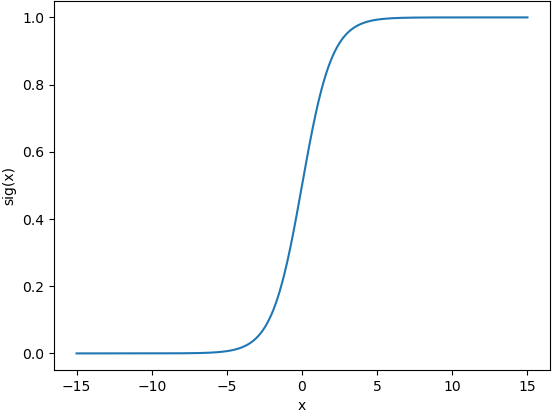
\includegraphics[width=0.4\textwidth]{pictures/sig_func.png}
		\caption{Graph der Sigmoidfunktion}
		\label{sig_func}
	\end{wrapfigure}

	Um aus diesem Netz Input nun die Aktivierung zu berechnen, benötigt man eine Aktivierungsfunktion, die dafür sorgt, dass die Aktivierung zwischen 0 und 1 liegt. Wir haben dafür eine Sigmoidfunktion benutzt, die eine Zahl nimmt und einen Wert zwischen 0 und 1 ausgibt (s. Abbildung \ref{sig_func}). Dies wird dann für jedes Neuron in jedem Layer wiederholt. Da man aber immer die Aktivierungen des vorherigen Layers benötigt, muss man das ganze vom Input Layer zum Output Layer machen. Daher auch der Name Forward Pass. Die Interpretation der Outputs hängt von den Trainingsdaten ab. Die allgemeine Formel für die Aktivierung eines Neurons lautet also:


	{\Large
	\[
		\sig(x)=\frac{1}{1+e^{-x}}
		\]
	\[
		a_{j} = \sig\left(\sum_{L} (a_{L} * W_{Lj}) + b_{j}\right)
		\]}
	
	\noindent wobei $a_j$ = die Aktivierung des Neurons $j$, $L$ = der vorherige Layer, $a_L$ = alle Aktivierungen des Layers $L$, $W_{Lj}$ = alle Gewichte zwischen dem Neuron $j$ und den Neuronen des Layers $L$, und $b_j$ = der Bias des Neurons $j$. \cite{brotcrunsher:forwardpass}	
	
	\threesub{Loss/Cost} 

	Um zu bestimmen, wie gut ein bestimmtes neuronales Netz ist, gibt es die sogenannte Cost-Funktion (auch Loss-Funktion genannt), die mithilfe von Trainingsdaten funktioniert.
	
	Trainingsdaten bestehen aus einer Liste aus Trainingsdatensätzen. Jeder dieser Datensätze beinhaltet Inputs für das Netzwerk und die richtigen Outputs dafür. Machine Learning, das mit solchen Trainingsdaten arbeitet, wird Supervised Learning genannt.

	Die Funktion für die Cost des Output-Layers und somit gesamten Netzwerkes (für einen Trainingsdatensatz) lautet wie folgt:

	{\Large \[
		C_0 = (a_L - y)^2
	\]}

	%C0 = (aL − y)2 

	\noindent wobei $C_0$ = die Cost des Output-Layers, $L$ = der letzte Layer (Output Layer), $a_L$ = die Aktivierungen des Layers $L$, und $y$ = die richtigen Outputs für die Inputs, mit denen die Aktivierungen berechnet wurden. 
	
	Um die Cost zu berechnen, muss man also für alle Output Neuronen die Differenz der gegebenen und der richtigen Aktivierungen bilden. Danach muss man diese Differenzen quadrieren und am Ende alle Ergebnisse aufsummieren. Dies kann man für alle Trainingsdatensätze wiederholen und von allen Costs den Durchschnitt nehmen, um die allgemeine Performance eines Netzwerkes zu überprüfen. Diese Art der Cost-Funktion wird mittlere quadratische Abweichung (mean squared error, kurz MSE) genannt. 
	
	Zusammenfassend kann man also sagen, dass die Cost die Abweichung von den berechneten und den richtigen Outputs angibt.
	
	Aufgrund des Trainingsdatensatzes weiß man nun, wie der Output Layer verändert werden
	muss.

	\threesub{Backpropagation}

	Doch wie verändert man nun die Aktivierungen des Output-Layers? Es müssen alle Gewichte und Biases davor angepasst werden. Um nun zu wissen, wie ein Gewicht verändert werden muss, gibt es folgende Funktion:

	{\Large \[
		\Delta W_{ij} = \epsilon * \delta_i * a_j
	\]}

	wobei $\Delta W_{ij}$ = um wie viel das Gewicht $W$ zwischen den Neuronen $j$ und $i$ verändert werden muss, $\epsilon$ = die Lernrate (meist ein kleiner Wert wie 0.001), $\delta_i \approx$ die Ableitung der Cost des Neuronen $i$ im Verhältnis zum Gewicht $W_{ij}$, und $a_j$ = die Aktivierung des Neurons $j$. Was dabei oft verwirrend ist: $j$ bezeichnet das Neuron, welches zuerst kommt, und $i$ das Neuron, welches danach kommt (Reihenfolge im Forward-Pass), obwohl es bei $W_{ij}$ andersherum steht.

	Für den Bias wird die gleiche Formel benutzt, mit der Ausnahme, dass $a_j$ immer 1 ist und so wegfällt. Der Grund dafür liegt darin, dass der Bias, wie in der Struktur beschrieben, eigentlich nur ein Gewicht ist, das mit einem Neuron verbunden ist, welches immer eine Aktivierung von eins hat.

	Um nun $\delta_i$ für den Output Layer zu berechnen, gibt es folgende Gleichung: 

	{\Large \[
		\delta_i = \sig '\left({\netin}_i\right) * (a_i (\textrm{soll}) - a_i (\textrm{ist})) 
	\]}

	wobei $\sig '(x)$ = die Ableitung von $\sig(x)$, also $\sig'(x) = \sig(x) * (1 - \sig(x))$, $\netin_i$ = der Netzinput des Neurons $i$, $a_i(\textrm{soll})$ = die Aktivierung, die das Neuron haben sollte (also das gleiche wie $y$), und $a_i(\textrm{ist})$ = die Aktivierung, die das Neuron hat.

	Mit dieser Formel wird berechnet, welche Aktivierung das Neuron haben sollte, was an $a_i(\textrm{soll}) - a_i(\textrm{ist})$ erkennbar ist. Die Aktivierungsfunktion mit dem Netz Input wird als Faktor mit einberechnet, da möglichst nur die Gewichte stark verändert werden sollen, die bei dem Trainingsdatensatz eine hohe Aktivierung haben, also durch diese Inputs besonders angesprochen werden. So werden zum Beispiel beim Sortieren nur die Neuronen miteinander verknüpft, die für ein bestimmtes Muster verantwortlich sind.
	
	Für die Neuronen der Hidden Layers muss man alle $\delta$'s des nächsten Layers mit den von dem Neuron dorthin führenden Gewicht multiplizieren und dann summieren. Dadurch werden die Änderungen, die die Aktivierungen dieser Neuronen brauchen ($\delta$), zusammengerechnet, da natürlich die Aktivierungen im nächsten Layer unterschiedliche Änderungen in dem gleichen Neuron benötigen.
	
	Durch die Multiplikation mit den dahin führenden Gewichten werden diese Änderungen gewichtet, da sie auf einige Neuronen größere Auswirkungen haben als auf andere. Wie beim Output Layer auch wird diese Summe noch mit $\sig'(\netin)$ multipliziert, um die Aktivierung durch bestimmte Muster angesprochener Neuronen noch weiter zu erhöhen und weniger/kaum angesprochener Neuronen zu senken, sodass die Ergebnisse besser und eindeutiger werden. Die Formel hierfür lautet:

	{\Large \[\sig'({\netin}_i) * \sum_{L}{\left(\delta_L\ast W_{Li}\right)}\]}

	\noindent wobei $L$ = der nächste Layer, $\delta_L$ = alle $\delta$'s des Layers $L$, und $W_{Li}$ = alle Gewichte, die ein Neuron des nächsten Layers und Neuron $i$ verbinden.


	Da immer die nächsten Layer und der Output Layer benötigt werden, ergibt es Sinn, diese Optimierung beim Output Layer zu starten und dann rückwärts die \mbox{$\delta$-Werte} für jeden Layer zu berechnen und für die nächsten Berechnungen zu speichern -- daher auch der Name Backpropagation. \cite{MITNeuronale} \cite{3b1b:fft} \cite{brotcrunsher:backwardpass}

	\threesub{Flux}

	Wir haben in unserem letzten Projekt bereits ein neuronales Netzwerk mit dieser Funktionsweise selbst programmiert, um es besser verstehen zu können \cite{AIComposer}. Für dieses Projekt haben wir allerdings das Package Flux benutzt, welches die gleichen oder besseren Ergebnisse liefern sollte, mit deutlich besserer Performance, da es stark optimiert und sehr weit entwickelt wurde.

	\subsubsection{Roboter}

	Für unseren Roboter haben wir uns entschieden, Lego Mindstorms EV3 Motoren zu benutzen, die von einem EV3-Brick gesteuert werden, der wiederum von einem Raspberry Pi 3B gesteuert wird (s. Abbildung \ref{robot-funktion} und \ref{Robot}). Der Grund dafür, dass wir keine Motoren direkt mit dem Raspberry Pi steuern, ist, dass wir schon alle Teile für einen EV3 Roboter haben. Somit müssten wir entweder neue Motoren kaufen oder passende Adapter finden, welche meist nur mit C und Python funktionieren und teuer sind.

	\begin{figure}[h!]
		\centering
		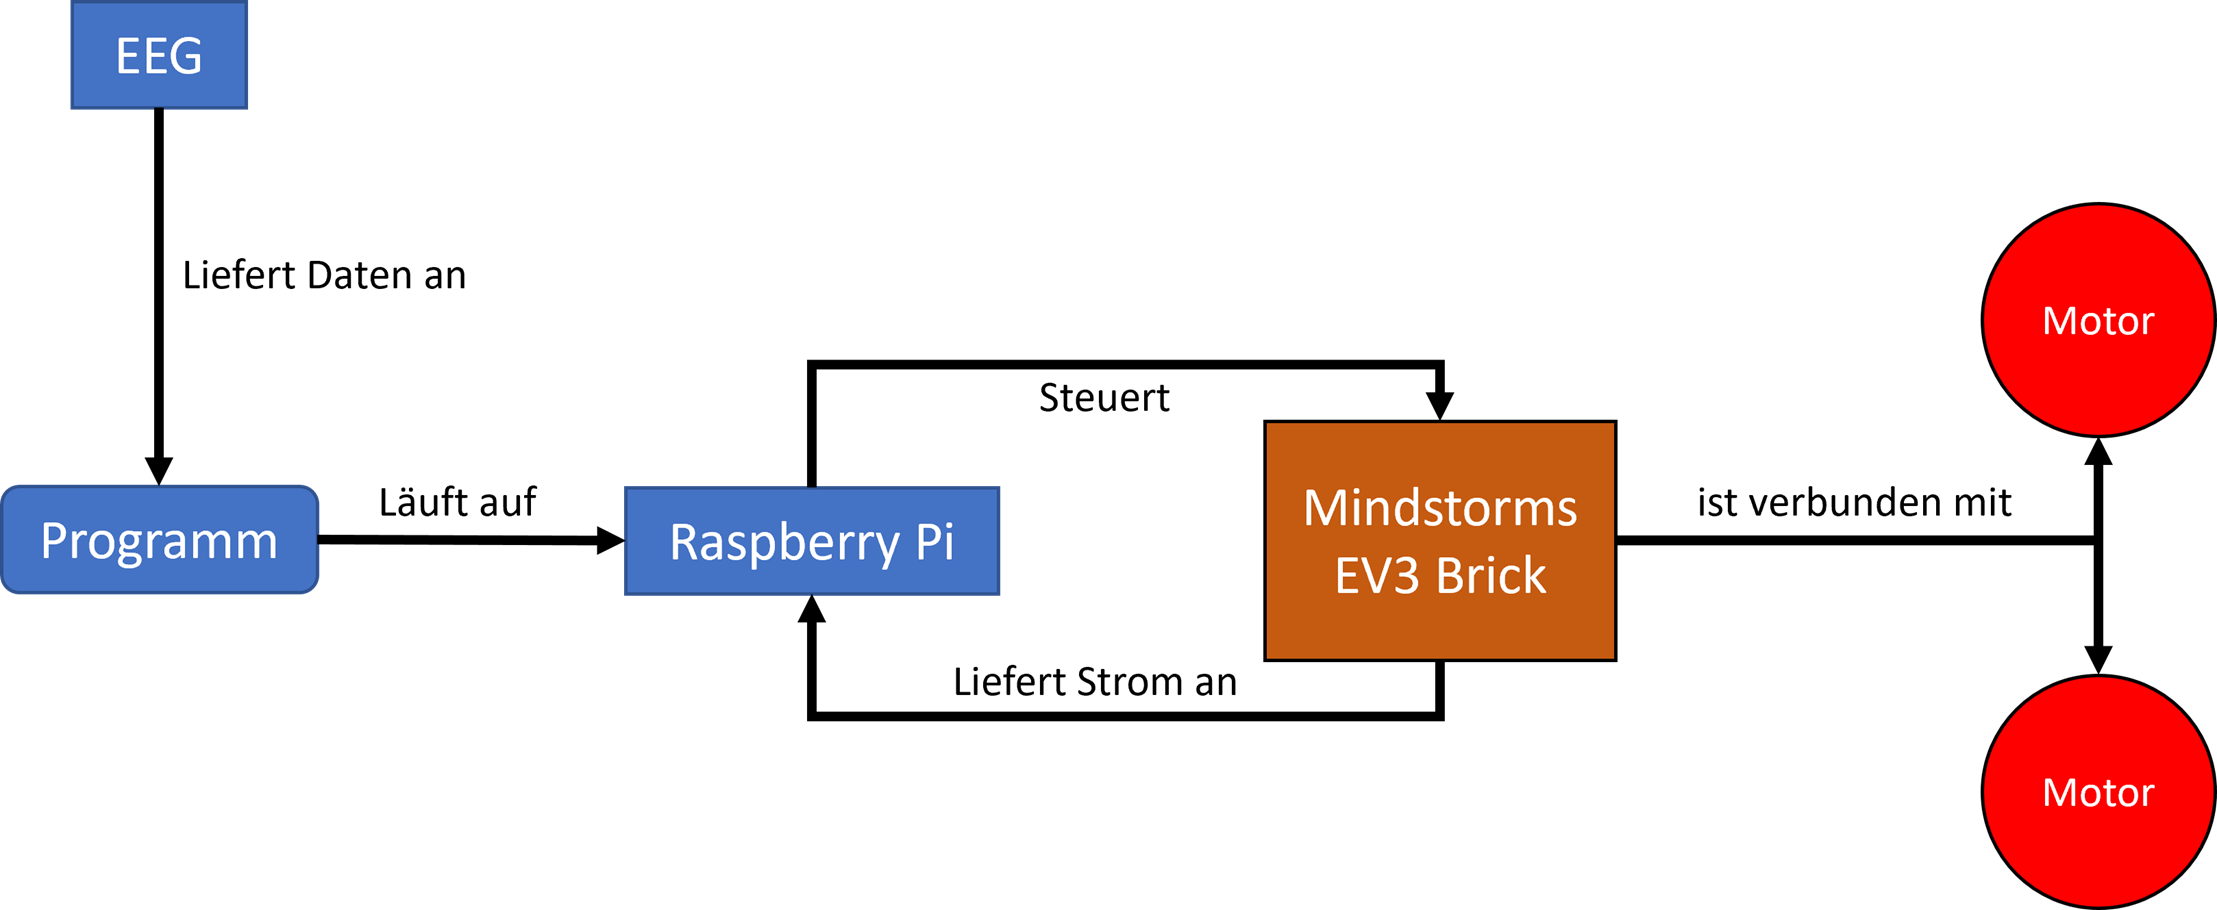
\includegraphics[width=0.8\textwidth]{pictures/roboter-funktionsweise.png}
		\caption{Ablauf von Gehirnaktivität zur Motorbewegung}
		\label{robot-funktion}
	\end{figure}

	Wir haben dafür das Package ev3dev.jl benutzt, welches wir bereits für die Robotik-AG programmiert hatten.

	Mehr technische Details zu der Umsetzung lassen sich beim GitHub Repository des Packages finden \cite{ev3dev}.

	\begin{figure}[H]
		\centering
		\includegraphics[width=0.5\textwidth]{pictures/roboter-annotated.png}
		\caption{Unser Roboter (ohne Raspberry Pi, der über den EV3-Brick gehört)}
		\label{Robot}
	\end{figure}


	\begin{figure}[h!]
		\centering
		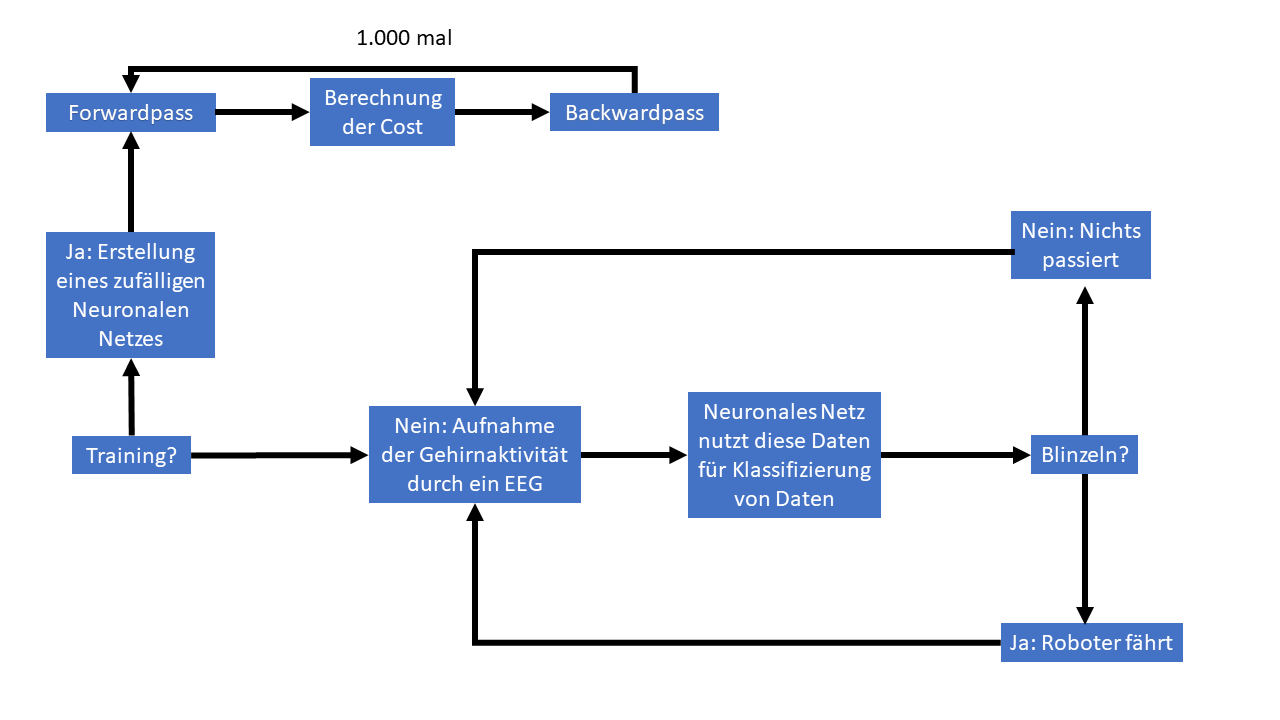
\includegraphics[width=0.9\textwidth]{pictures/Abbildung-des-Programms.png}
		\caption{Funktionsweise des Programms}
		\label{Gesamtfunktion}
	\end{figure}

	%\newpage
	%\subsection{Funktionsweise des Programms}

	%\begin{figure}[h!]
	%	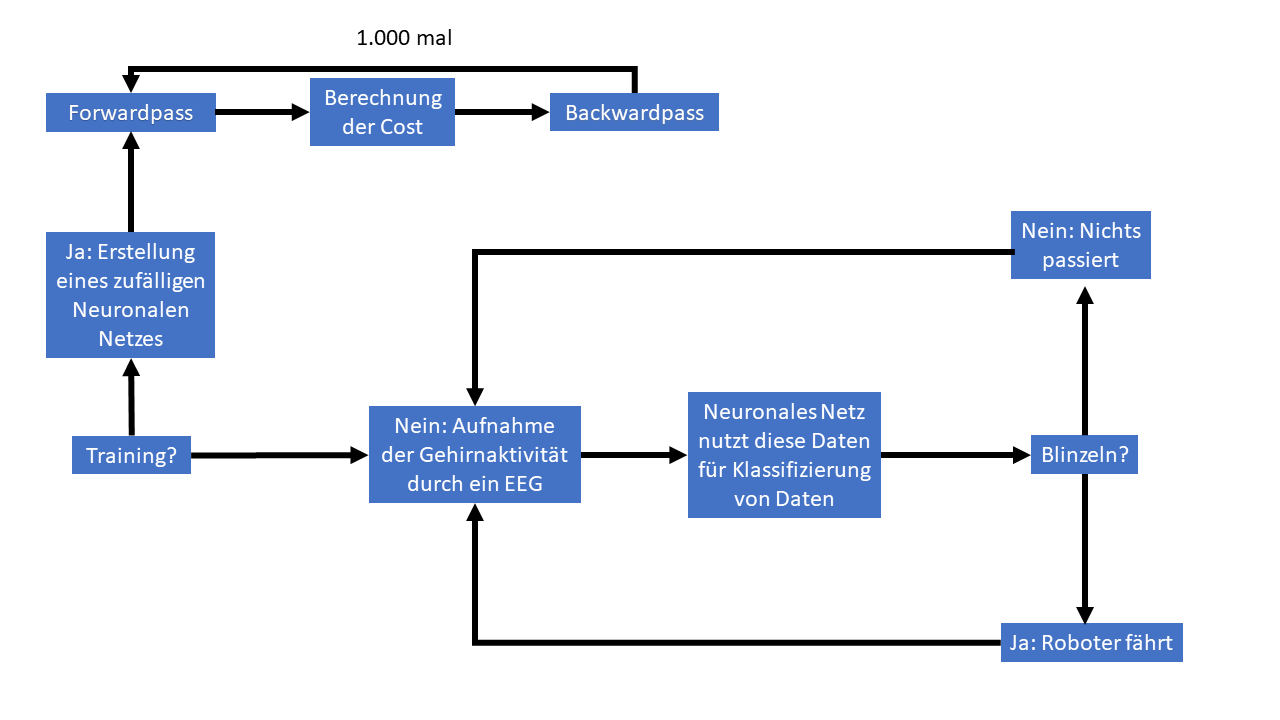
\includegraphics[width=\textwidth]{pictures/Abbildung-des-Programms.png}
	%	\caption{Funktionsweise des Programms}
	%\end{figure}

	\section{Ergebnisse}

	{\textbf{Der gesamte Code kann auf unserem GitHub Repository gefunden werden! \cite{InterpretingEEG}} }

	Zuerst haben wir versucht, eine KI zu trainieren, welche erkennen kann, ob eine Person gerade geblinzelt hat oder nicht. Diese könnte man zum Beispiel nutzen, indem man einen Roboter immer dann nach vorne fahren lässt, wenn eine Versuchsperson blinzelt.

	Wir haben uns für ein neuronales Netzwerk entschieden, welches als Input eine Sekunde an EEG-Daten nimmt, da sich die Auswirkungen von Blinzeln ungefähr für diesen Zeitraum in den EEG-Daten abbilden. Bei diesem Versuch haben wir keine Fourier Transformation benutzt.

	Als Outputs haben wir uns für zwei Neuronen entschieden. Dabei stehen die Werte jeweils für die Sicherheit des Netzwerkes, dass geblinzelt oder nicht geblinzelt wurde.

	Unsere Trainingsdaten bestehen dann aus 200 dieser Datensätze, 100 davon mit Blinzeln und 100 ohne. Unser Netzwerk haben wir aber nur mit 90\% dieser Datensätze (180) trainiert, damit wir mit den restlichen 20 kontrollieren konnten, ob das Netzwerk auch unbekannte Daten richtig verarbeiten kann.

	Für den Aufbau der Hidden Layer des Netzwerkes haben wir uns entschieden, da wir mehrere verschiedene Ansätze ausprobiert haben und diese Struktur konsistent die besten Ergebnisse geliefert hat. Die Struktur ist zu sehen in Abbildung \ref{NetzStruktur}.

	\begin{figure}[h!]
		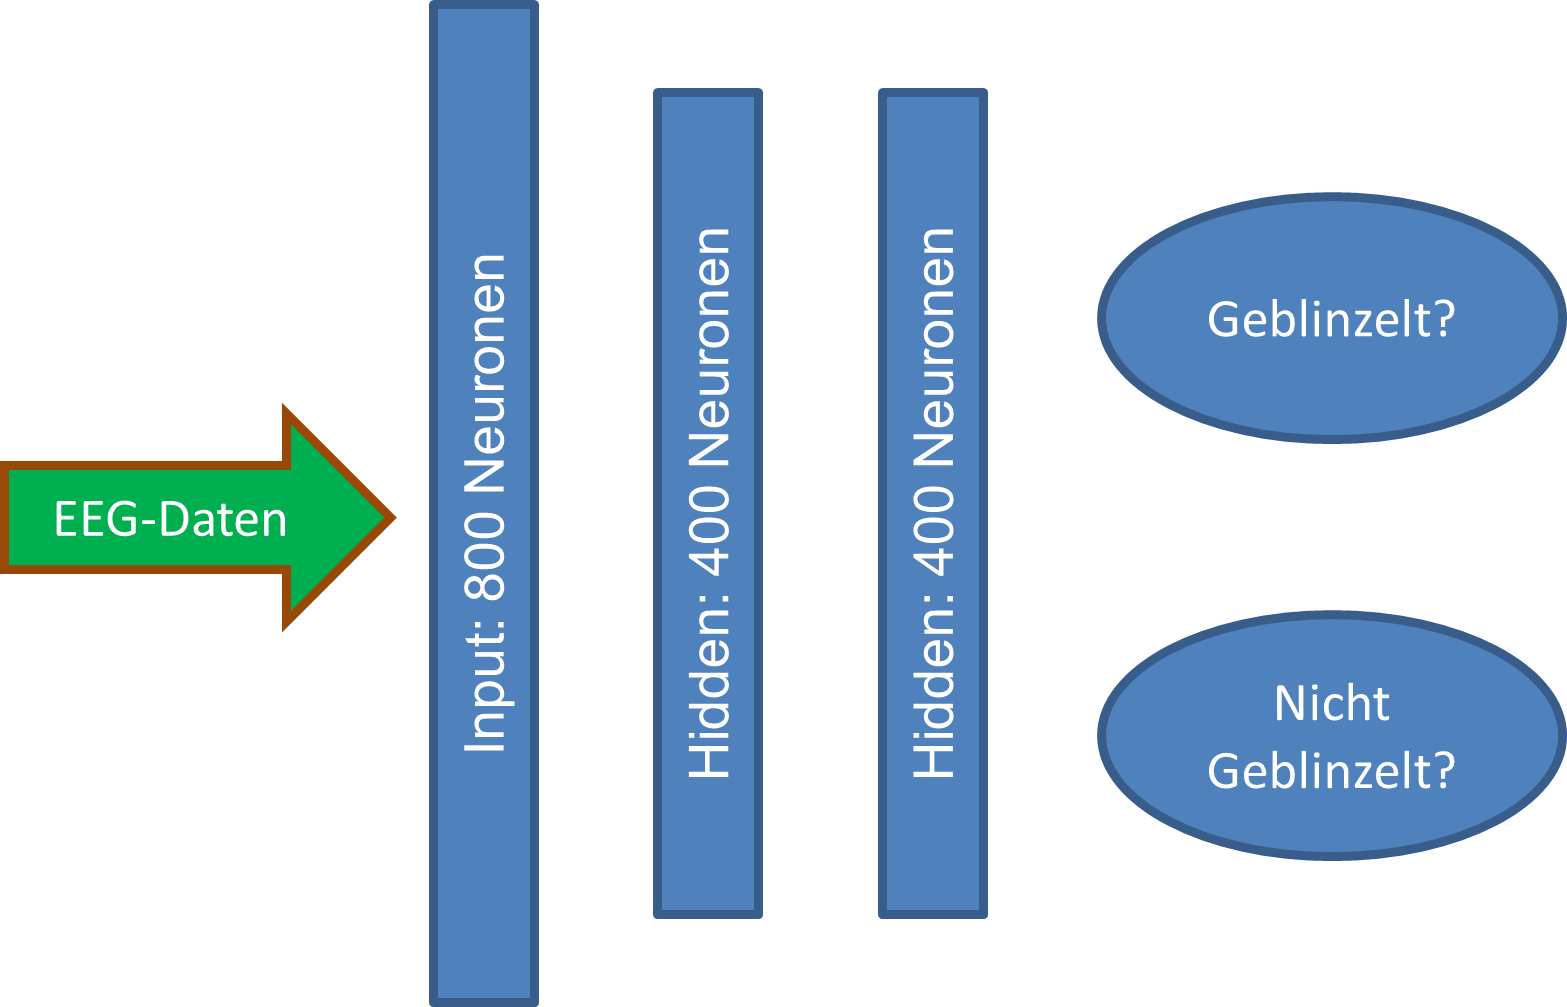
\includegraphics[width=0.75\textwidth]{pictures/netzwerk-struktur.png}
		\caption{Struktur unseres neuronalen Netzwerks}
		\label{NetzStruktur}
	\end{figure}

	Das Ergebnis war positiv:

	\begin{figure}[h!]
		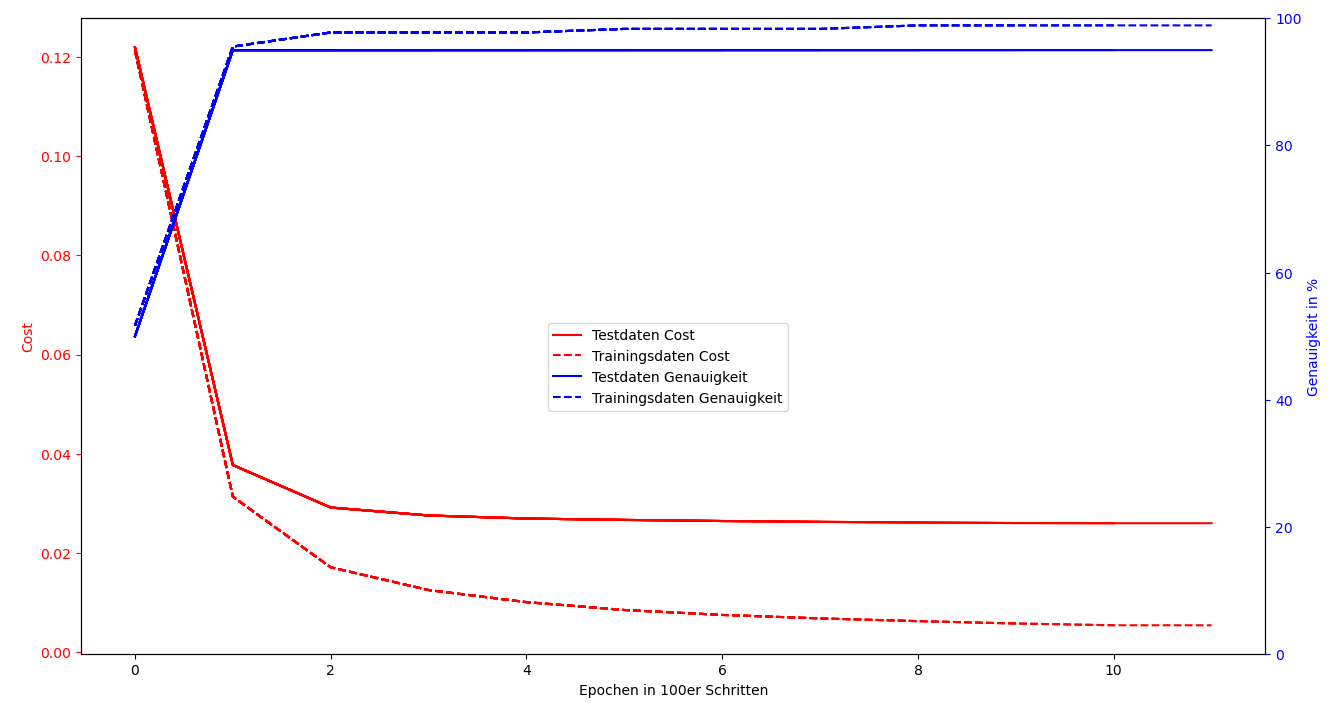
\includegraphics[width=\textwidth]{pictures/training-nofft.png}
		\caption{Der Cost- und Genauigkeitsverlauf der Test- und Trainingsdaten beim Trainieren des Netwerkes ohne FFT}
		\label{training-nofft}
	\end{figure}

	Wie man an Abbildung \ref{training-nofft} sehen kann, erreichte das neuronale Netzwerk in diesem Fall in nur 1000 Epochen (ca. 5 Minuten Rechenzeit) eine Genauigkeit von 95\%, bei anderen Durchläufen erhielten wir auch 100\%.

	Bei dem Versuch mit Frequenzfiltern durch FFT war die Struktur ähnlich, die Menge an Neuronen in jedem Layer wurde jedoch halbiert, da es nur 100 Inputs gibt, weil die Fast Fourier Transformation bei einer zeitlichen Auflösung von 200 Hertz nur 1 - 100 Hertz berechnen kann. Wir erhielten bei der gleichen Zahl an Wiederholungen (\enquote{Epochen}) ähnliche Ergebnisse (s. Abbildung \ref{training-fft}).

	\begin{figure}[h!]
		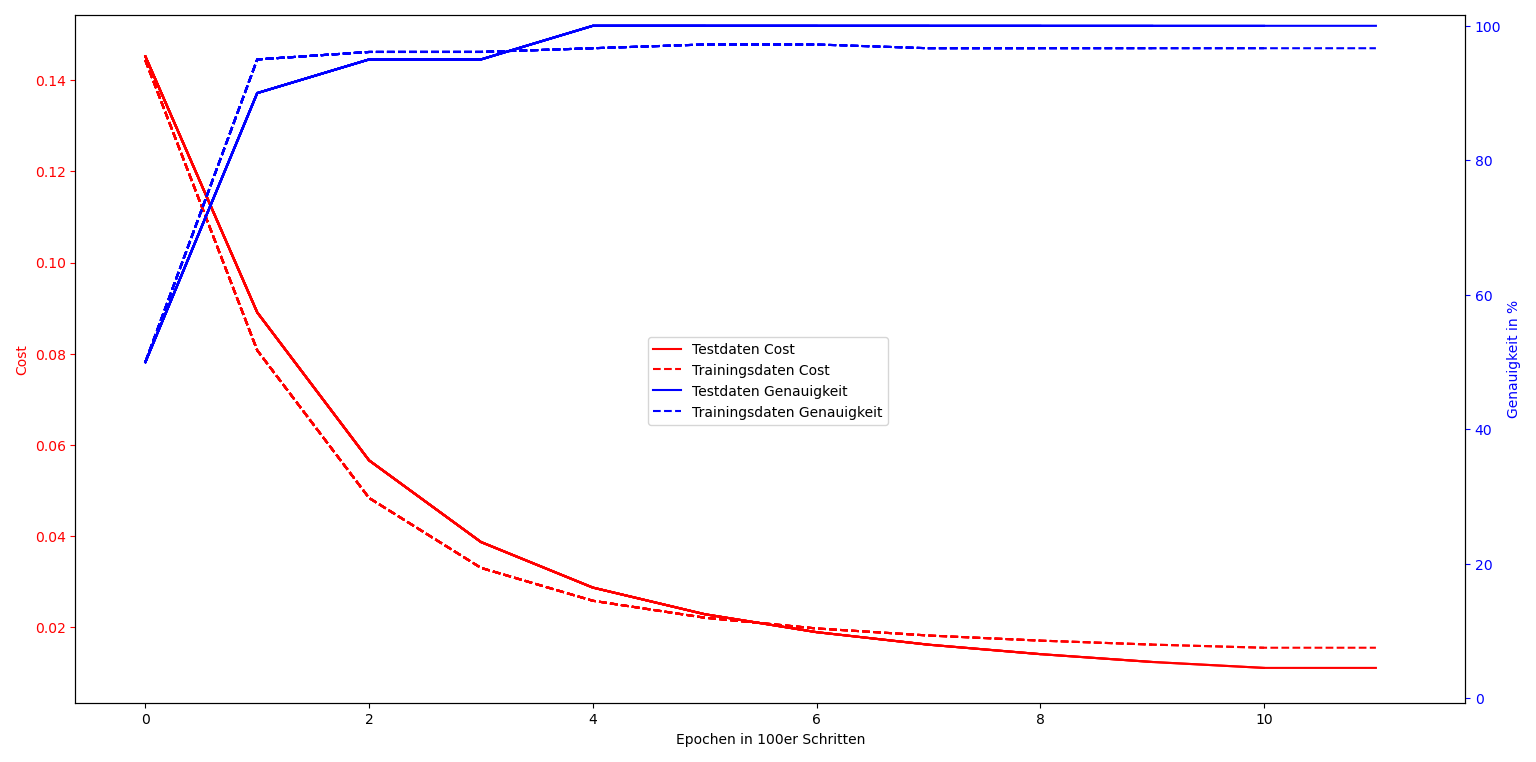
\includegraphics[width=0.9\textwidth]{pictures/training-fft2.png}
		\caption{Der Cost- und Genauigkeitsverlauf der Test- und Trainingsdaten beim Trainieren des Netwerkes mit FFT}
		\label{training-fft}
	\end{figure}

	Dies heißt, dass die FFT wie erwartet die Ergebnisse nicht verschlechtert hat. Jedoch lässt sich auch nicht genau sagen, inwiefern sie besser ist als keine. Denn die kleinen Erfolgs-Unterschiede, die man oft sieht, wie hier auch, stammen meist davon, dass jedes neuronale Netzwerk zufällig initialisiert wird und somit, selbst mit einem ansonsten identischen Verfahren, einen leichten Unterschied in den Ergebnissen zeigen kann.

	Zu Beginn hatten wir ein noch größeres Problem: Die Testdaten konnten sicher erkannt werden, aber als wir es mit neuen Daten von anderen Personen und in anderen Räumen versuchten, hat das Netzwerk meist komplett versagt.

	Das Ziel der allgemeinen Anwendung war also nicht gegeben gewesen. 

	Dieses Problem konnten wir allerdings lösen, indem wir einen größeren Raum benutzt und mehr Daten gesammelt haben. So gab es eine größere Diversität an Daten und das neuronale Netzwerk wurde darauf trainiert, auf die Umgebung zurückzuführende Veränderungen zu ignorieren.

	Das neuronale Netzwerk konnte Blinzeln danach sicher erkennen. Wie in Abbildung \ref{test-graph} zu erkennen ist, war die Differenz zwischen den beiden Output-Neuronen als nicht geblinzelt wurde fast 1, bei kräftigem Blinzeln auch. Die Klassifizierung des Netzwerks war also mit sehr großer Sicherheit getätigt worden. Bei leichtem Blinzeln hat das erste Output-Neuron (geblinzelt, grüner Graph) das zweite (nicht geblinzelt, roter Graph) zwar nicht oder nur leicht übertroffen, war aber dennoch klar erkennbar.

	\begin{figure}
		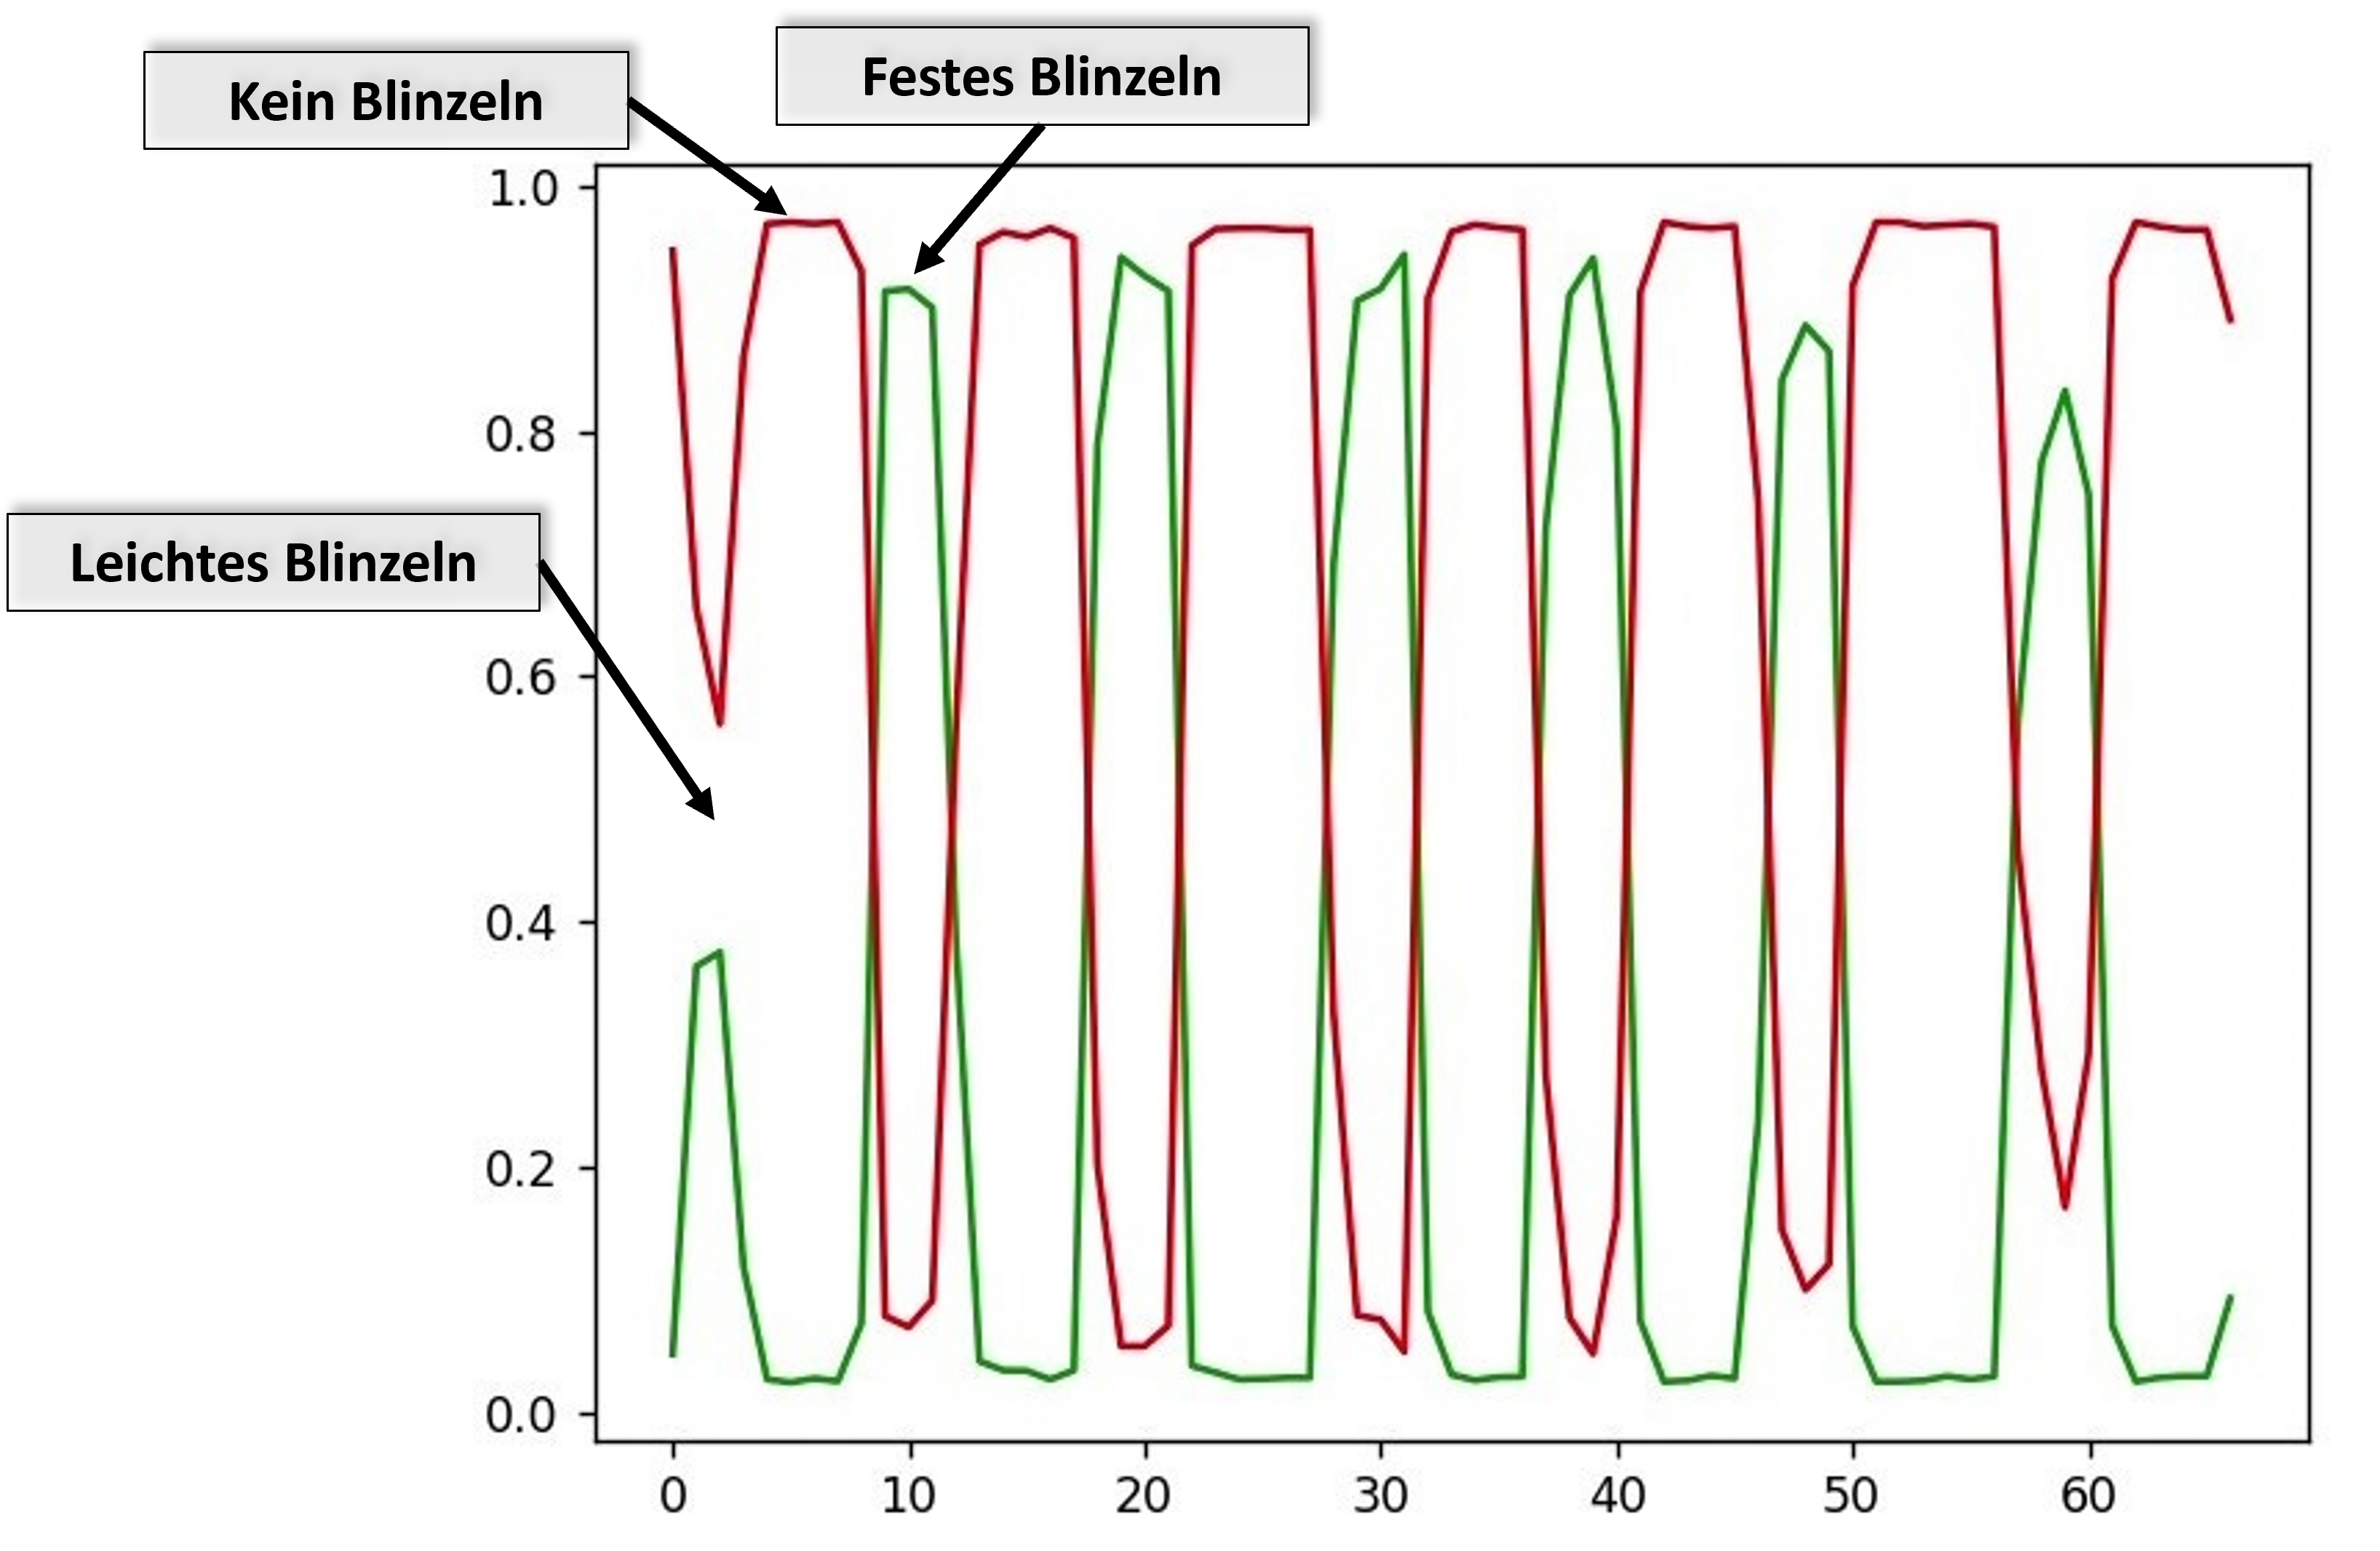
\includegraphics[width=\textwidth]{pictures/Test-Graph-annotated.png}
		\caption{Ein Live-Test unseres Projektes, die grüne Linie repräsentiert das erste Output-Neuron (Sicherheit, dass geblinzelt wurde), die rote das zweite Output-Neuron (Sicherheit, dass nicht geblinzelt wurde). Die x-Achse ist die Zeit in 0,25 Sekunden Schritten}
		\label{test-graph}
	\end{figure}

	Es fällt auch auf, dass die Summe der beiden Output-Neuronen stets ungefähr 1 ergibt und die Graphen sich an y = 0.5 grob spiegeln. Wir vermuten, dass beim neuronalen Netz entweder nur einer der Werte ausgerechnet wird und der andere der Umkehrwert dessen ist $\left(1 - P\right)$, oder beide fast identisch berechnet werden.
	
	Ein Video mit Aufnahme der Augen, des Graphen, und des Roboters ist auf YouTube verfügbar \cite{projekt-video}.

	Im Video und auch als Testperson merkt man, dass eine Verzögerung kaum spürbar ist. Grund dafür ist vermutlich, dass die KI für diese Tests alle 0,25 Sekunden das EEG der letzten Sekunde abgefragt  haben. Somit gibt es nicht eine maximale extra Verzögerung von z.B. \qty{1000}{\milli\second}, sondern nur \qty{250}{\milli\second}.

	\section{Diskussion}

	Wir sind zufrieden damit, dass wir unser erstes Teilziel erreicht haben:

	Der Roboter fährt sicher, und es gibt kaum eine Verzögerung.

	Die Kosten der benutzten Hardware halten sich noch in Grenzen: Beim Kauf hat die gesamte EEG-Ausstattung ca. 550€ gekostet, was zwar eigentlich eine hohe Summe ist (danke an den Förderverein für die Finanzierung!), aber \enquote{professionelle} Ausrüstung kostet deutlich mehr.

	Die Performance des Programms kann außerdem zwar noch verbessert werden, jedoch dauern beim Trainieren 1000 Epochen (genug für ca. 100\% Genauigkeit) auf dem Test-System bereits lediglich 5 Minuten. 

	Als ersten folgenden Schritt wollen wir zuerst die aktuell offenstehenden Fragen beantworten, indem wir das Trainieren mit nur einem Output-Neuron ausprobieren und recherchieren, warum unsere Ergebnisse in großen Räumen und draußen so viel besser waren als in kleinen Räumen.

	Außerdem könnte man die Signalqualität des EEG noch verbessern, indem man Elektrodengel aufträgt. 

	Der nächste, große Schritt wird dann sein, die Elektroden an anderen Positionen anzubringen, wo sie nicht mehr auf Muskeln sitzen und wir somit kein EMG mehr benutzen, sondern ein tatsächliches EEG.

	Wir planen dafür, den Okzipitalen Kortex (mittig am Hinterkopf, leicht über dem Inion) zu verwenden. Denn Professor Everling hat uns informiert, dass dort $\alpha$-Wellen (7 - 13 Hertz) besonders stark ausgeprägt sind, und er hat uns den Tipp gegeben, dass unser EEG vor allem diesen Frequenzbereich gut aufnehmen könnte. Dies hat sich bereits bestätigt, denn wie man in Abbildung \ref{EEG-FFT} sehen kann, ist der niedrige Frequenzbereich zumindest beim Blinzeln am stärksten ausgeprägt.

	Zudem wollen wir in fernerer Zukunft versuchen, mithilfe unseres neuronalen Netzes bereits bei allen Menschen vorhandene, selbst kontrollierbare Gehirnaktivität zu finden und sicher zu erkennen, jedoch ohne vorherige Konditionierung. Solche Gehirnaktivität könnte z.B. der allgemeine Gedanke an \enquote{Rechts} sein, was womöglich mit erhöhter Aktivität auf der linken Hirnhälfte in Verbindung stehen könnte.
	
	\section{Danksagung}

	\subsection{Finanzierung} \label{Foerderverein}

	Danke an den Förderverein \enquote{Gesellschaft der Freunde des Gymnasium Eversten e.V.} für die Finanzierung des EEG-Geräts. Alle finanzierten Teile sind in der \hyperref[Materialien]{Materialliste} mit $\star$ gekennzeichnet. 

	\subsection{Unterstützung}

	Vielen Dank an Professor Everling vom \enquote{The Brain and Mind Institute} der Western University in Kanada, der uns geholfen hat, einen Ansatz in diesem komplizierten Thema zu finden und praktische Tipps zum Umgang mit dem EEG gegeben hat. \footnote{\href{https://www.uwo.ca/bmi/investigators/stefan-everling.html}{https://www.uwo.ca/bmi/investigators/stefan-everling.html}}

	Dank geht auch an Ino Saathoff, der für uns die Hülle der EEG-Platine mit seinem 3D-Drucker erstellt hat.

	Natürlich geht auch Dank Oliver Samkovskij und Ino, die zusammen mit uns den Roboter gebaut haben.

	\section{Quellen \& Referenzen}

	\printbibliography[title={Literatur}, keyword={Literatur}, notkeyword={YTVideos}]

	\printbibliography[title={Videos}, keyword={YTVideos}]

	\printbibliography[title=Programme, keyword=Programme]

\end{document}